\documentclass{article}
\usepackage[czech]{babel}
\usepackage[utf8]{inputenc}
\usepackage{graphicx}
\usepackage{pdfpages}
\usepackage{textgreek}
\usepackage{xargs} 
\usepackage{xcolor}
\usepackage{pdfpages}
\usepackage[colorinlistoftodos,prependcaption,textsize=tiny]{todonotes}
\newcommandx{\xtodo}[2][1=]{\todo[linecolor=red,backgroundcolor=red!25,bordercolor=red,#1]{#2}}


\usepackage{listings}
\usepackage{color}

\definecolor{dkgreen}{rgb}{0,0.6,0}
\definecolor{gray}{rgb}{0.5,0.5,0.5}
\definecolor{mauve}{rgb}{0.58,0,0.82}

\lstset{frame=tb,
	language=Sql,
	aboveskip=3mm,
	belowskip=3mm,
	showstringspaces=false,
	columns=flexible,
	basicstyle={\small\ttfamily},
	numbers=none,
	numberstyle=\tiny\color{gray},
	keywordstyle=\color{blue},
	commentstyle=\color{dkgreen},
	stringstyle=\color{mauve},
	breaklines=true,
	breakatwhitespace=true,
	tabsize=3
}




\begin{document}
	
	
	%---------------------------------------------------------------------------------------------------------------------------------------------------------------%
	
	
	\begin{titlepage}	
		\begin{center}
			
\includegraphics[width=5cm]{logo.jpg}\\[3.5cm]
			{\Huge KIV/VSS}\\[0.5cm]
			{\Large 1.9. – Generování náhodných čísel}\\[0.5cm]
			{\large  Gaussovské rozdělení}\\[4.5cm]
			{\large  Miroslav Liška – A17N0081P}\\[0.5cm]
			{\large  topiker@students.zcu.cz}\\[0.5cm]
			{\large   9.12.1992}\\[0.5cm]
			\vfill
			
			{\large \today}
			
		\end{center}
	\end{titlepage}
	
	
	
	\section{Zadání} %%%%%%%%%%%%%%%%%%%%%%%%%%%%%%%%%%%%%%%%%%%%%%%%%%%%%%%%%%%%%%%%%%%%%%%%%%%%%%%%%%%%%%%%%%%%%%%%%%%%%%%%%%%%%%%%%%%%%%%%%%%%%%%%%%%%%%%%%%
	\setcounter{page}{1}
	
	\subsection{Teoretické pozadí}
	Zejména při fyzické aktivitě nebo příjmu potravy dochází k výrazné změně koncentrace glukózy.
	V zadaných datech máte několik měření koncentrací glukózy v intersticiální tekutině [mmol/l].
	Jsou vzorkovaná po 5 minutách tzv. systémem CGMS. 
	U každého měření je časová značka a měření jsou rozdělena do segmentů, které trvají od několika hodin do několika dní. 
	Vaším úkolem je identifikovat cca 3 - 5 významných kolísání koncentrací glukózy během dne (uvažuje se 3 jídlo a 2 fyzická zátěž). 
	Při identifikaci si můžete pomoci i časovými značkami, případně naměřenou koncentrací v krvi, která by po jídle a při fyzické aktivitě měla být taktéž zvýšená.
	
	V běžném životě si pacient údaje o jídle a fyzické aktivitě zadává manuálně a ještě s chybou. 
	Systém automatické detekce by tuto chybu redukoval a napomohl tak lepší léčbě pacienta. 
	Práce tedy není "šuplíková", ale má praktické využití (cca každý 11. člověk má diabetes a polovina z nich o tom ani neví, protože diabetes nebolí, dokud není pozdě).
	
	Změny koncentrace glukózy lze nejjednoduššeji detekovat jako ohodnocené plovoucí okno - tj. fixní časový úsek, který bude "plout" v čase segmentu od jeho počátku až na konec.
	Ohodnocení okna může být součet rozdílů koncentrací glukózy v daném okně.
	S algoritmem lze dále experimentovat, např. velikost okna a mezní ohodnocení (tj. od kdy je okno považováno za významnou změnu koncentrace glukózy) lze určovat např. pomocí Diferenciální evoluce, nebo jiným algoritmem - může to být i 2D půlení intervalu. 
	Vlastní invenci při vývoji detekčníh algoritmu se meze nekladou.
	
	\subsection{Verze úlohy}
	Zpracujte úlohu alespoň ve dvou verzích ze tří možných:
	
	\begin{itemize}  
		\item Paralelní program pro systém se sdílenou pamětí
		\item x86 CPU + OpenCL/C++ AMP GPGPU
		\item Paralelní program pro systém s distribuovanou pamětí
	\end{itemize}
	
	
	\subsection{Data}
	%%%%%%%%%%%%%%%%%%%%%%%%%%%%%%%%%%%%%%%%%%%%%%%%%%%%%%%%%%%%%%%%%%%%%%%%%%%%%%%%%%%%%%%%%%%%%%%%%%%%%%%%%%%%%%%%%%%%%%%%%%%%%%%%%%%%%%%%%%
	Naměřené hodnoty jsou uloženy ve formátu SQLite verze 3.
	Konkrétně jsou uloženy v tabulce measuredvalue. 
	Požadované hodnoty najdete ve sloupci ist, který vyjadřuje koncetraci v intersticiální tekutině v [mmol/l]. 
	Čas měření je zanesen ve sloupci measuredat, a je ve formátu ISO 8601. Data jsou seskupena do tzv. segmentů, viz  sloupec segmentid. 
	Naměřená data zpracovávejte vždy po celých segmentech. 
	Jméno segmentu lze dohledat  v tabulce timesegment a jméno pacienta analogicky v tabulce subject.
	
	\subsection{Výstup}
	%%%%%%%%%%%%%%%%%%%%%%%%%%%%%%%%%%%%%%%%%%%%%%%%%%%%%%%%%%%%%%%%%%%%%%%%%%%%%%%%%%%%%%%%%%%%%%%%%%%%%%%%%%%%%%%%%%%%%%%%%%%%%%%%%%%%%%%%%%
	Na stdout vypište získané statistické ukazatele jako tabulku v csv formátu. 
	Zároveň vygenerujte grafický výstup ve formátu SVG (pro každý segment jedno SVG), ve kterém graficky znázorníte změny koncentrace glukózy považované za příjem potravy, fyzickou aktivitu, apod. 
	Implentujte přepínač, který buď segment vykreslí v celé jeho délce, anebo ho bude zalamovat po 24 hodinách - tj. osa X (čas) bude mít hodnoty od 00:00 do 23:59. 
	V takovém případě by mohlo být vidět, např. zda pacient snídán či večeří pravidelně - což je také možná nápověda pro detekční algoritmus.
	
	\subsection{Další statistiky}
	%%%%%%%%%%%%%%%%%%%%%%%%%%%%%%%%%%%%%%%%%%%%%%%%%%%%%%%%%%%%%%%%%%%%%%%%%%%%%%%%%%%%%%%%%%%%%%%%%%%%%%%%%%%%%%%%%%%%%%%%%%%%%%%%%%%%%%%%%%
	Program také spusťte s jedním vláknem/procesem a změřte čas výpočtu sériovým kódem a čas výpočtu paralelizovaným kódem (pro všechny verze paralelizovaného kódu zvlášť). 
	Z těchto hodnot vypočítejte následující ukazatele:
	
	\begin{itemize}  
		\item Amdahlův zákon, $f$ -- čas sériově prováděné části kódu
		\item Gustafsonův zákon, $a$ -- část kódu, kterou nelze paralelizovat
		\item Karp-Flattova metrika, $e$ -- část sériově prováděného kódu
	\end{itemize}
	\newpage
	\section{Analýza}
	%%%%%%%%%%%%%%%%%%%%%%%%%%%%%%%%%%%%%%%%%%%%%%%%%%%%%%%%%%%%%%%%%%%%%%%%%%%%%%%%%%%%%%%%%%%%%%%%%%%%%%%%%%%%%%%%%%%%%%%%%%%%%%%%%%%%%%%%%%
	\subsection{Detekce změn koncentrace glukózy}
	O chování koncentrace glukózy v krvi víme (informace z přednášek), že pokud pozorovaný subjekt zkonzumuje nějakou potravinu, konentrace vzroste. 
	Pokud je subjektem vynaložena nějaká aktivita, koncentrace typicky mírně vzroste a pak začne klesat. Tyto akty pak v datech generují významné kolísání, jejichž detekce je cílem práce. Dále je z přednášky známo, že kolísání trvá typicky tři hodiny s tím, že nárůst trvá hodinu a následné klesání pak dvě hodiny. 
	
	Jedním z možných řešení detekce je nalezení lokálních extrémů. Následně se pro každý extrém vezmou spojitě data začínající před extrémem a po extrému o nějaké velikosti. Pro výběr nejlepších výsledků je nutné získané intervaly ohodnotit. Dále je potřeba nějakým způsobem naložit s překrývajícími se intervaly, například jejich sloučením či vyřazením horšího.
	
	Dalším řešením může být evoluční genetický algoritmus. 
	Data jsou rozdělena náhodně na intervaly o pevné velikosti a pro každý interval je vypočítána jeho fitness funkce. Následně se vybrané intervaly posunou a spočítá se jejich fitness funkce a tím vznikne nová generace intervalů. Podle chování genetického algoritmu se s novou generací patřičně naloží. Posouvání probíhá do té doby, dokud nevznikne nejlepší generace intervalů, které jsou pak detekovaným kolísáním.
	
	\subsubsection{Zvolené řešení}
	\label{sec:zvoleneReseni}
	Pro detekci kolísání jsem se rozhodl použít algoritmus posuvného okénka. Princip spočívá v tom, že se napříč daty iteruje tzv. okénkem o velikosti n. Každá iterace posune okénko o jedno měření dál. Každé okénko je ohodnoceno funkcí. 
	V implementaci je jako funkce zvoleno rozdíl sousedních hodnot na druhou. 
	Na druhou z toho důvodu, aby nebylo okénko ohodnoceno záporně. 
	
	Jakmile je spočítáno ohodnocení všech okének, je potřeba vybrat pouze ty nejlepší a nějakým způsobem naložit s okénkami, které se překrývají. Při výběru významějších okének jsem se rozhodl vybrat pouze ty, jejichž ohodnocení je lepší, než průměrná hodnota.
	Po výběru významějších okének je možné, že se budou jednotlivé intervaly překrývat. Je předpokladem, že ve vybraná okénka budou reprezentovat části s významným klesáním či nárůstem. Pokud se tedy intervaly překrývají, je vhodné je spojit. Pro takto spojená okénka znovu spočítáme jejich ohodnocení a následně se vezme n nejlepších.
	\subsection{Načtení uložených dat}
	
	Naměřené hodnoty jsou ve formátu SQLite verze 3. Pro přístup k datům je tedy vhodné přistoupit za pomocí SQL dotazů. Při analýze bylo zjištěno, že ne všechny segmenty uvedené v tabulce segmentů mají i naměřená data a naopak nějaká naměřená data mají id segmentu, které není v tabulce segmentů. Při načtení dat z databáze budou tedy zvolena pouze ta data, jejichž id segmentu odpovídá tabulce segmentů.
	Pro práci hledání kolísání bude nutné, aby data byla seřazena podle data měření (measuredate). Datum měření je uloženo ve formátu ISO 8601. Podle doporučení je dobré převést datum na formát, kdy hodnota 1.0 představuje datum 1.1.1900.
	\subsection{Paralelizace}
	 Na obrázku \ref{fig:flowdiagram} je možné vidět průběh výpočtu a interakcí programu. Slovně byl popsán v sekci \ref{sec:zvoleneReseni}
	 
	Pro parelelizaci této úlohy jsem si vybral paralelizaci se sdílenou pamětí a paralelizaci na GPGPU.
	
	Pravděpodobně nejlepším řešením bude paralelizace na úrovni segmentů, tedy detekce kolísání jednotlivých segmentů bude probíhat současně. Důvodem výběru tohoto místa je, že se jedná o práci s větším množstvím nezávislých dat, tedy by režie spojená s paralelizací nemusel být zpomalující.
	Další možností paralelizace je paralelizace uvnitř segmentu na úrovni jednotlivých dní. Jednalo by se tak o paralelizaci uvnitř paralelizace (segment a jednotlivé dny). Vzhledem k tomu, že počet dat uvnitř jednotlivých dní je nízký (maximálně několik stovek), je předpokladem, že tato paralelizace přínos nepřinese. Tento přístup ale bude v rámci experimentu implementován.
	
	Vzhledem k charakteru zvoleného algoritmu (mnoho podmínek, porovnávání) a obecně nízkému počtu dat, se kterými se provádí matematické operace, je předpokladem, že paralelizace na GPGPU bude spíše zdržující.
	
	
\begin{figure}
	\centering
	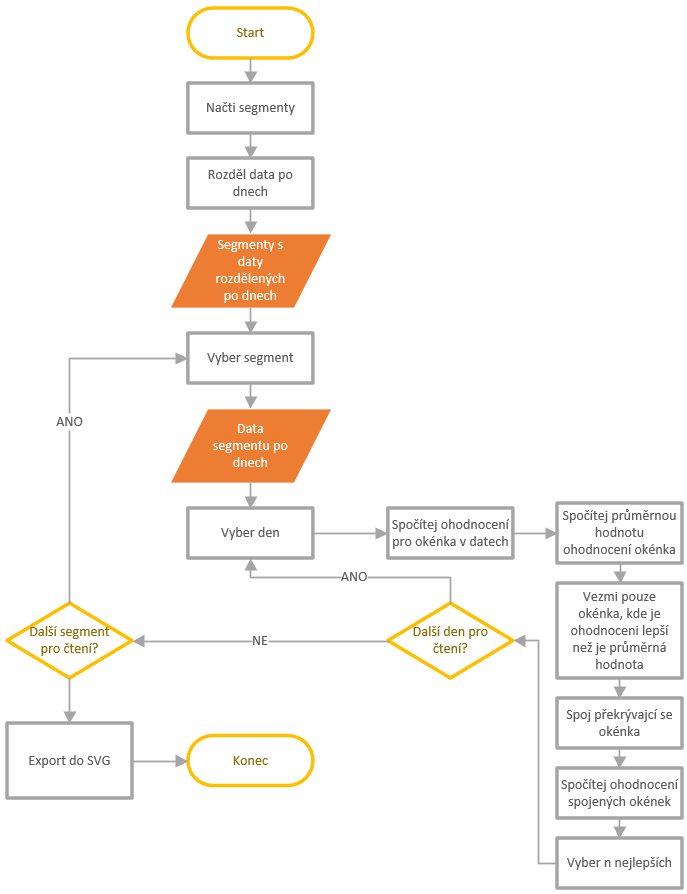
\includegraphics[width=0.7\linewidth]{flowDiagram}
	\caption[Flowdiagram programu]{Flowdiagram programu}
	\label{fig:flowdiagram}
\end{figure}

	\section{Programátorská dokumentace}
	%%%%%%%%%%%%%%%%%%%%%%%%%%%%%%%%%%%%%%%%%%%%%%%%%%%%%%%%%%%%%%%%%%%%%%%%%%%%%%%%%%%%%%%%%%%%%%%%%%%%%%%%%%%%%%%%%%%%%%%%%%%%%%%%%%%%%%%%%%
	
	\section{Závěr} %%%%%%%%%%%%%%%%%%%%%%%%%%%%%%%%%%%%%%%%%%%%%%%%%%%%%%%%%%%%%%%%%%%%%%%%%%%%%%%%%%%%%%%%%%%%%%%%%%%%%%%%%%%%%%%%%%%%%%%%%%%%%%%%%%%%%%%%%%
	
	
\end{document}